%!TEX root = ../data-imputation.tex
\section{Results}
\label{sec:results}

\felix{
\begin{itemize}
\item in the conclusion we should relate the performance to the training and prediction time and comment on the (large) differences - for AutoKeras, a lot more tuning is performed and we don't know whether it would have worked as well with less tuning.
\item we should highlight the limitations of our results (only one column, maybe too simple)
\item we should highlight the main findings; as far as i can see this would be: a) classical methods perform best (on these simple (?) data sets) and b) downstream performance is improved by X \% in Y \% of the experiments (we can use the quantiles in the boxplots) whereas when the imputation methods are trained on incomplete data, we cannot expect improvements.
\end{itemize}
}

In this section, we describe and visualize the results of our experiments.



\subsection{Experiment 1: Imputation Quality}

In this experiment we evaluate the imputation performance of each method when training on fully observed data and incomplete data.

Our goal was to provide as broad an overview as possible of the performance of various imputation methods. Therefore, we included a large number of datasets in our selection, with different data and task types. To make the results comparable this heterogeneous selection of data sets and tasks, we decided to aggregate the ranks of each imputation method in each experimental condition. Each condition is a combination of data set, corrupted column in a data set, missingness pattern and missingness ratio. The best rank is thus one, the worst rank six. For numerical columns the rank is is based on RMSE where lower is better. For categorical columns the rank is based on the F1 macro score where higher is better. Imputation methods with equal performance are assigned the same rank. If an imputation method produced Null-values we set its rank to be the last.

\subsubsection{Scenario 1: Training on Complete Data}

\begin{figure}\centering
    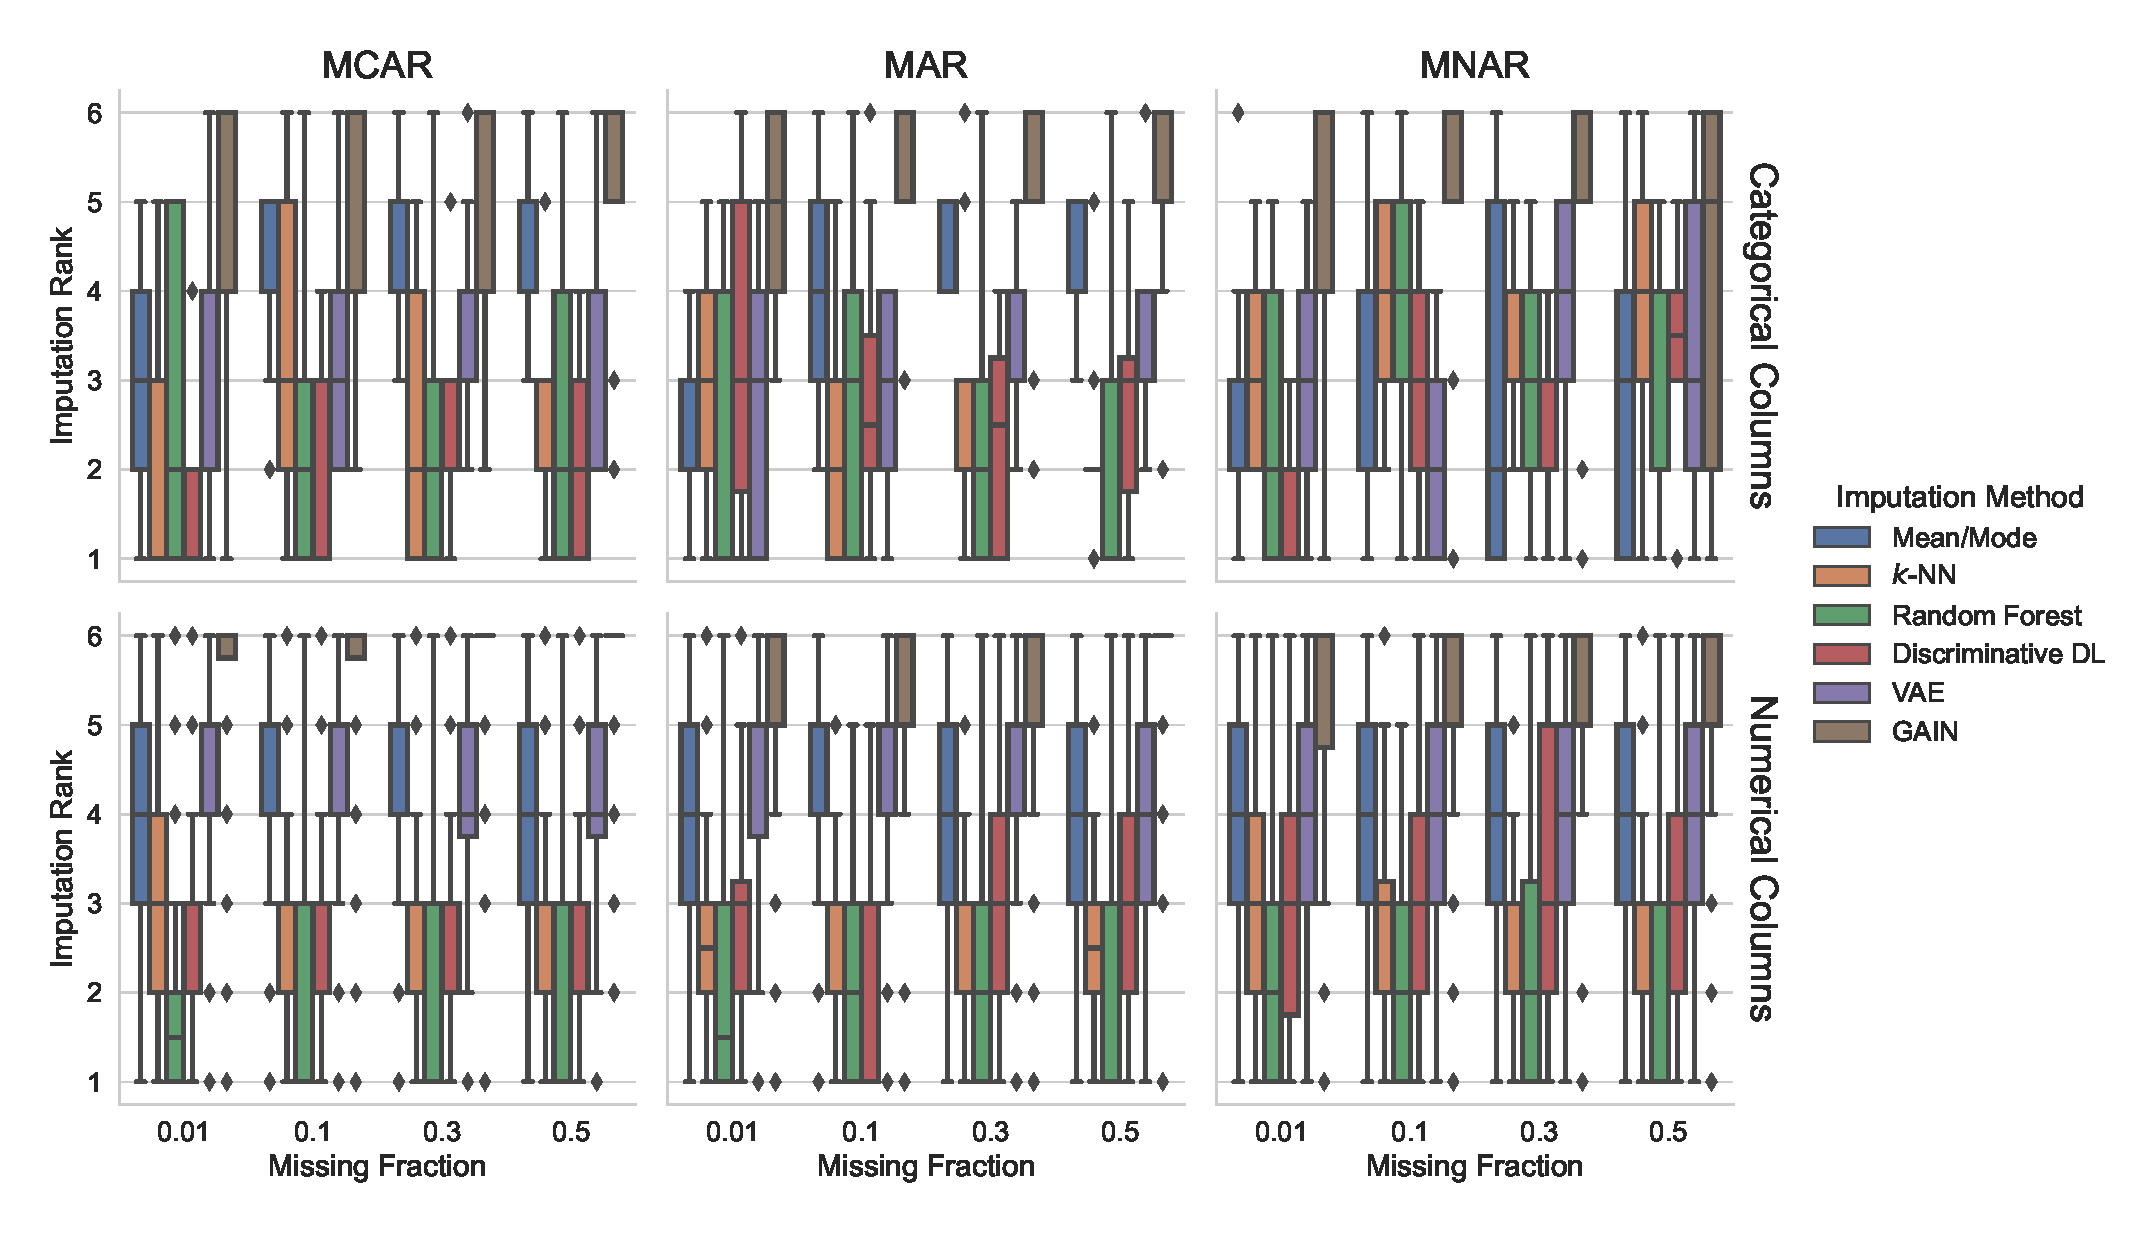
\includegraphics[width=1\columnwidth]{fully_observed_impute_rank_boxplot.eps}
    \caption[Imputation Ranks - Fully Observed]{In this figure, we visualize the results of \textit{Experiment 1} (imputation quality) in the \textit{Scenario 1} setting (training on complete data). The imputation rank is plotted against the missingness fraction. The plot is divided into six sub-plots, with three columns determined by the missingness type, ordered by task difficulty from easiest to most difficult (MCAR, MAR, MNAR). The first row shows imputation performance for categorical missing values,  the second row shows imputation performance for numerical columns. Within a single sub-plot, each box represents the distribution of ranks of each imputation method over all corresponding datasets/columns. Classical ML methods and discriminative DL tend to perform best. For categorical columns, however, there is often no improvement over Mode imputation, especially in the MNAR setting.
	}
	\label{fig:fully_observed_impute_rank_boxplot}
\end{figure}

\autoref{fig:fully_observed_impute_rank_boxplot} shows the aggregated ranks for imputation performance when imputation methods are trained on fully observed data.
When imputing categorical columns, there is no clear winner. However, the Discriminative Deep Learning approach (AutoKeras) yields high imputation quality in most cases. In the MAR setting, also the classical ML methods (Random Forest and k-NN) are among the first two to three ranks often times. With increasing complexity the DL based methods seem to improve. Notablyl Mean/Mode imputation compares favourably in many cases especially in the most complex MNAR setting. One method, the GAN based generative Deep Learning approach GAIN, appeared to perform worse than others in most cases. In the setting of highest complexity (MNAR with 50\% missing values) the results are not significantly worse than the other methods.

When imputing numerical columns the differences are more pronounced. Random Forest is the only method with 50\% of values among the first three ranks through all experimental conditions. However, the whiskers indicate that there are also some results ranging on the middle and even last ranks. k-NN and Discriminative DL are almost as strong with the boxes indicating many second and third ranks, with k-NN performing a bit better. Mean/Mode and VAE are in the middle with the former in being slightly in the lead. Again, GAIN performs worst, this time even more clearly.

To summarize, classical ML methods and discriminative DL perform best when imputing missing values. However, for categorical columns there is often no improvement over Mode imputation. The generative methods are mostly outperformed even by Mean/Mode with VAE not as clearly as GAIN.


\subsubsection{Scenario 2: Training on Incomplete/Imputed Data}


\begin{figure}\centering
    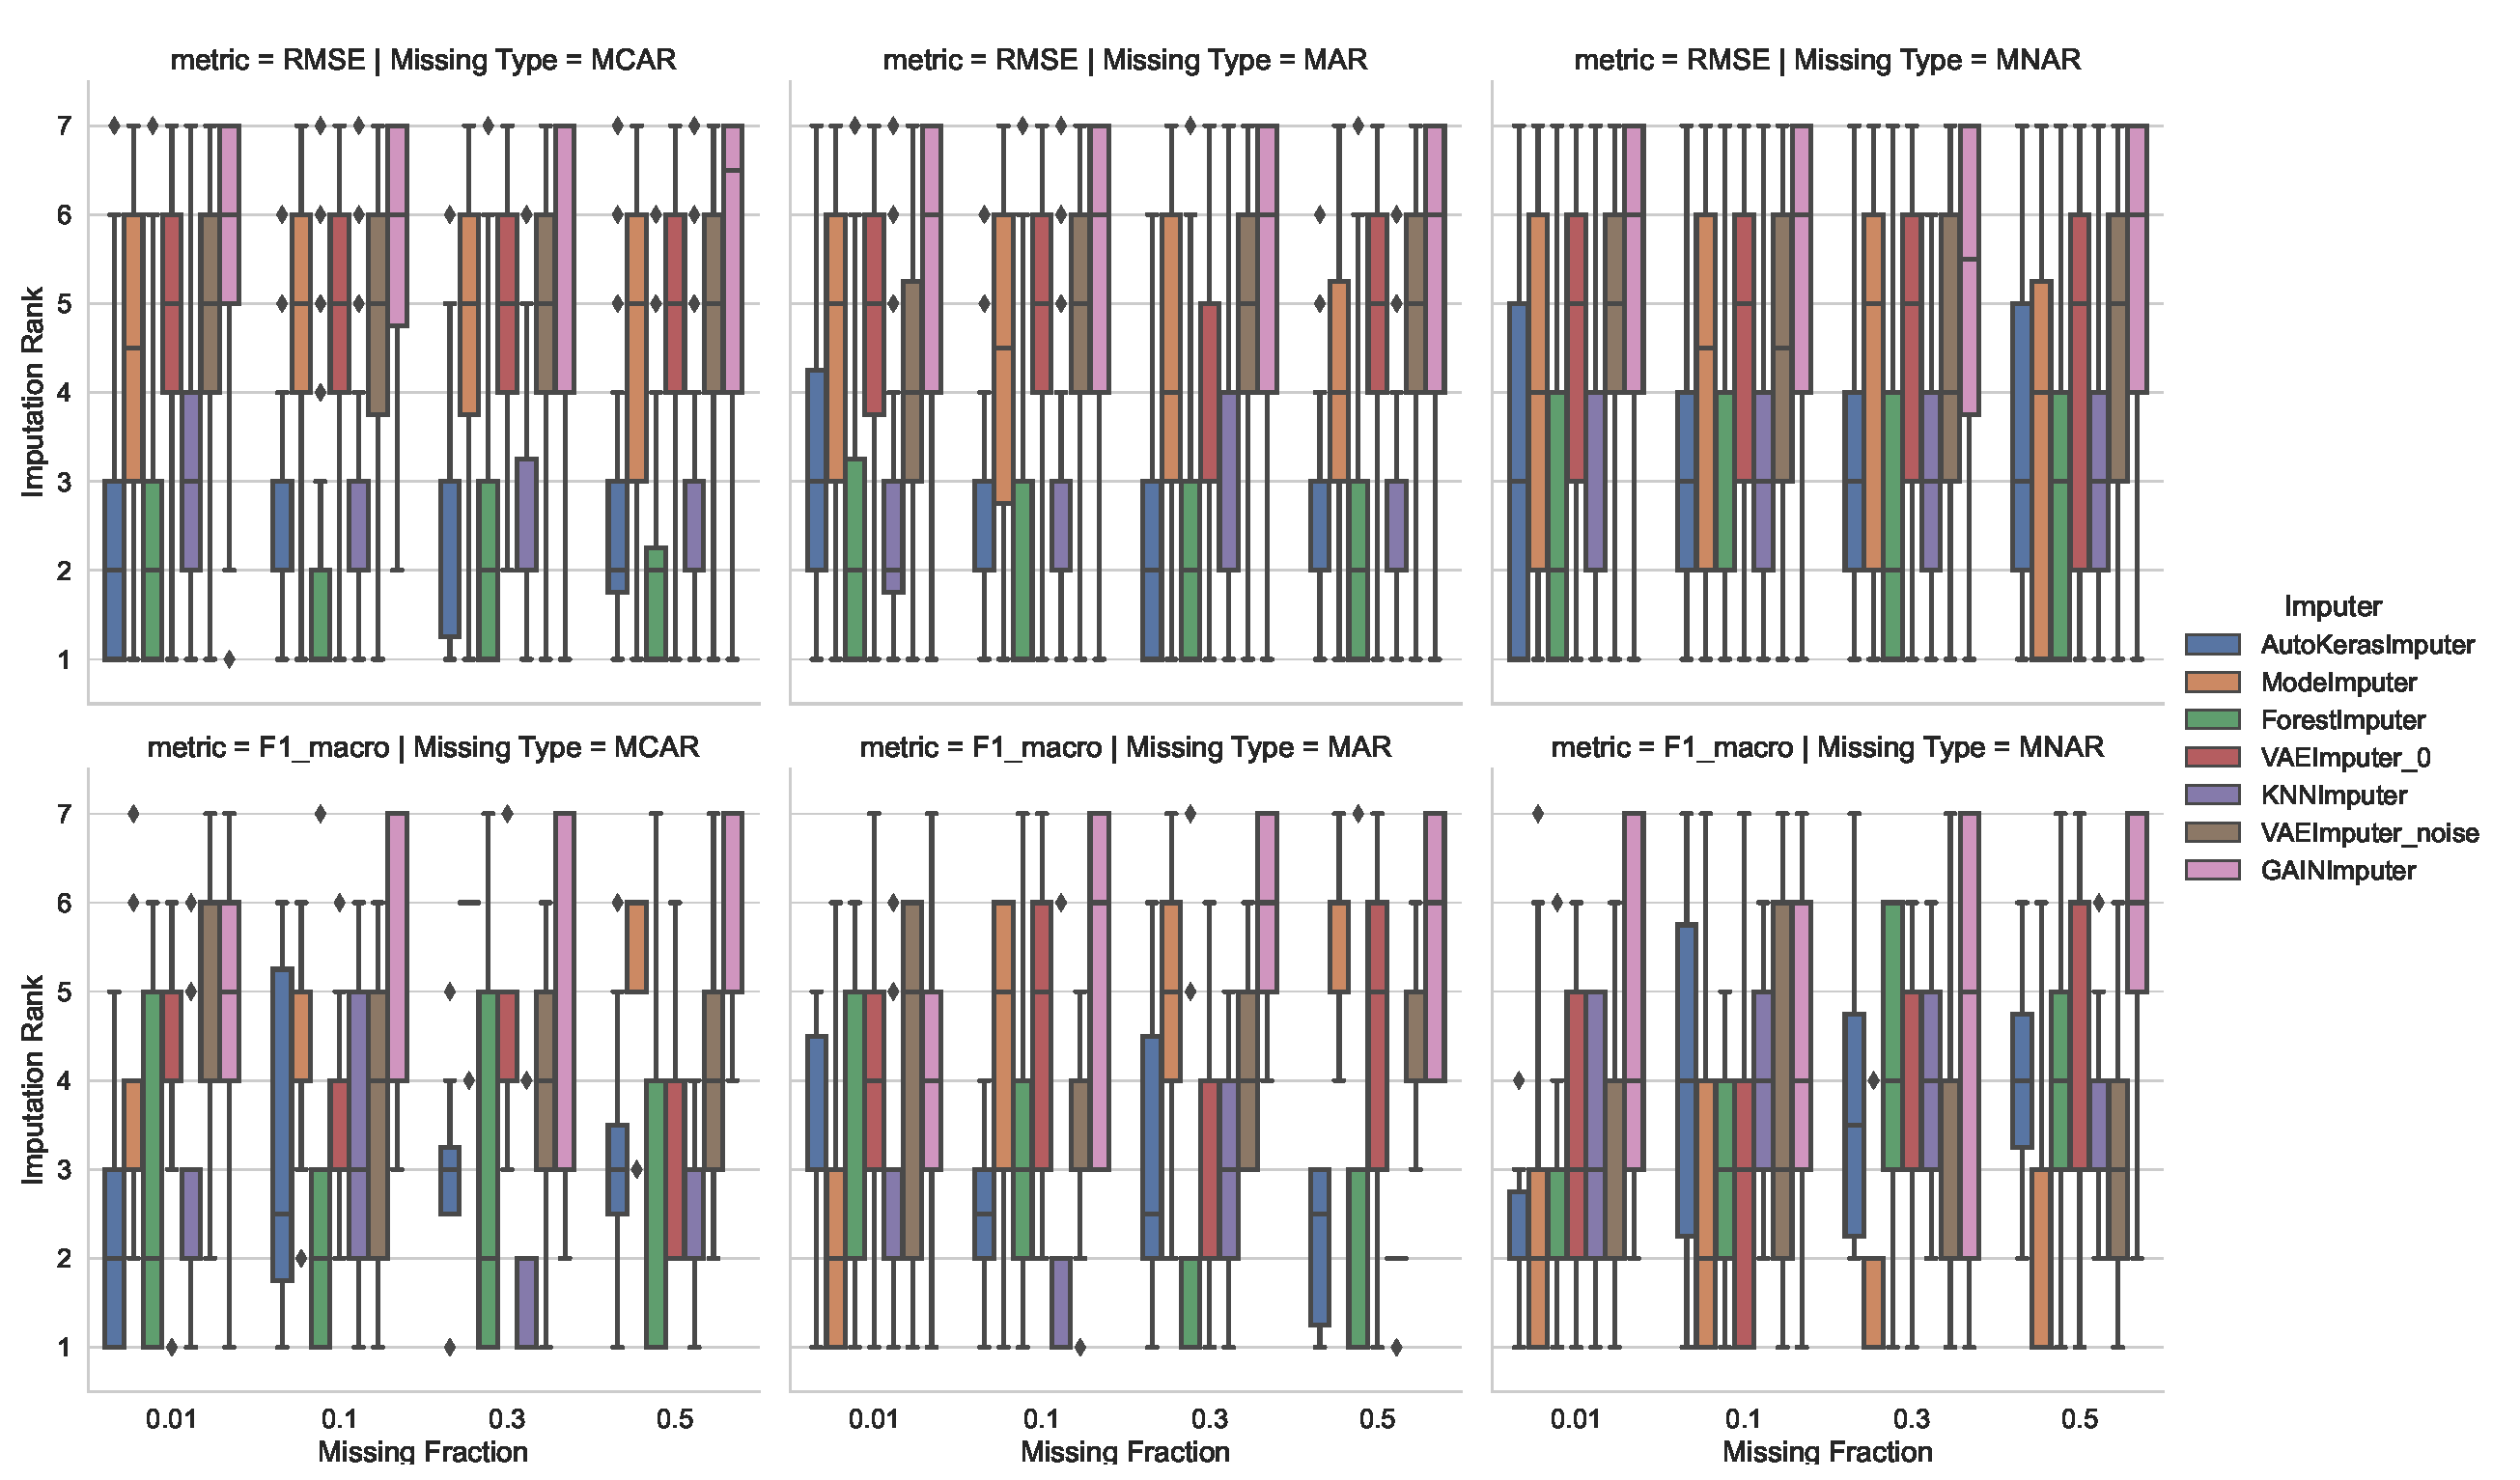
\includegraphics[width=1\columnwidth]{corrupted_impute_rank_boxplot.eps}

    \caption[Imputation Ranks - Corrupted]{Results of \textit{Experiment 1} (imputation quality) in the \textit{Scenario 2} setting (training on incomplete/imputed data). The imputation rank is plotted against the missingness fraction. The plot is divided into six sub-plots, with three columns determined by the missingness type, ordered by task difficulty from easiest to most difficult (MCAR, MAR, MNAR). The first row shows imputation performance for categorical missing values,  the second row shows imputation performance for numerical columns. Within a single sub-plot, each box represents the distribution of ranks of each imputation method over all corresponding datasets/columns. Classical ML methods and discriminative DL tend to perform best. For categorical columns, however, there is often no improvement over Mode imputation, especially in the MNAR setting.
    }
	\label{fig:corrupted_impute_rank_boxplot}
\end{figure}

\autoref{fig:corrupted_impute_rank_boxplot} shows the imputation performance in \textit{Scenario 2}, i.e. when training on incomplete/imputed data. For categorical columns it is even harder to find clear patterns. With increasing task difficulty, the performance of the Mode imputation increases, though with higher variance. Interestingly, Mode imputation outperforms other methods especially in the most challenging settings (MNAR with 30\% and 50\% missing values). The classical ML methods (k-NN and Random Forest) compare favourably in the MCAR and MAR setting, but Random Forest has much higher variance. Discriminative DL yields similar perforamance in these settings, slightly worse on average and with lower variance than Random Forest. For MCAR and MAR these three methods tend to yield better imputation performance than simply using Mode, especially with an increasing fraction of missing values. The generative models tend to perform worst, especially GAIN.

Similar to the fully observed training case, imputation on numerical columns yields a clearer ranking than for categorical missing values. The classical models yield best performances with a tendency of Random Forest to outperform k-NN, with larger variance of Random Forest. The Discriminative DL approach yields similar performance to the classical ML approaches in the MCAR and MAR settings. In the more challenging MNAR setting it performs slightly worse. Mean imputation and VAE perform comparably but worse than k-NN and Random Forest. GAIN falls on the last rank in most cases also in this setting.

Overall, the results of \textit{Scenario 1} (Figure \ref{fig:fully_observed_impute_rank_boxplot}) and \textit{Scenario 2} (Figure \ref{fig:corrupted_impute_rank_boxplot}) for numeric columns are quite similar. GAIN has become somewhat better in Scenario 2, although it still ranks worst. For categorical columns, the visualizations of the two scenarios are more pronounced in the incomplete training data setting. However, there are no major shifts in which the median worsens by more than two ranks. \arndt{Die letzte Aussage müssten wir prüfen, das geht aus den Plots nicht eindeutig hervor.}

We attribute the poor performance of GAIN in part to its numerical instability. Out of our 828 runs per imputation method GAIN failed 273 times, which amounts to 33\% of the cases. In those cases GAIN was assigned the last rank.

\subsubsection{Conclusions}
\felix{conclusions should be in the conclusions section, i guess?}
\arndt{nur eine temporäre sammlung von ideen}

- higher variance of random forest over knn due to outliers ?!

- generative methods mostly worse than mean/mode

- discriminative often as good as classical ML and better than mean/mode, but when considering the runtime might not be a good choice



\subsection{Experiment 2: Impact on Downstream Task}

In this experiment we evaluate the downstream performance of each method when training on fully observed data and incomplete data.

In \textit{Scenario 1} we use the definition for \textit{impact on downstream task} from \autoref{eq:impact}. In contrast, for \textit{Scenario 2} we use the slightly different definition from \autoref{eq:impact_scenario2}. Both of theses metrics are labeled \textit{Improvement} and the values represented on the Y-axis in \autoref{fig:fully_observed_downstream_boxplot} and \autoref{fig:corrupted_downstream_boxplot}.


\subsubsection{Scenario 1: Training on Complete Data}


\begin{figure}\centering
	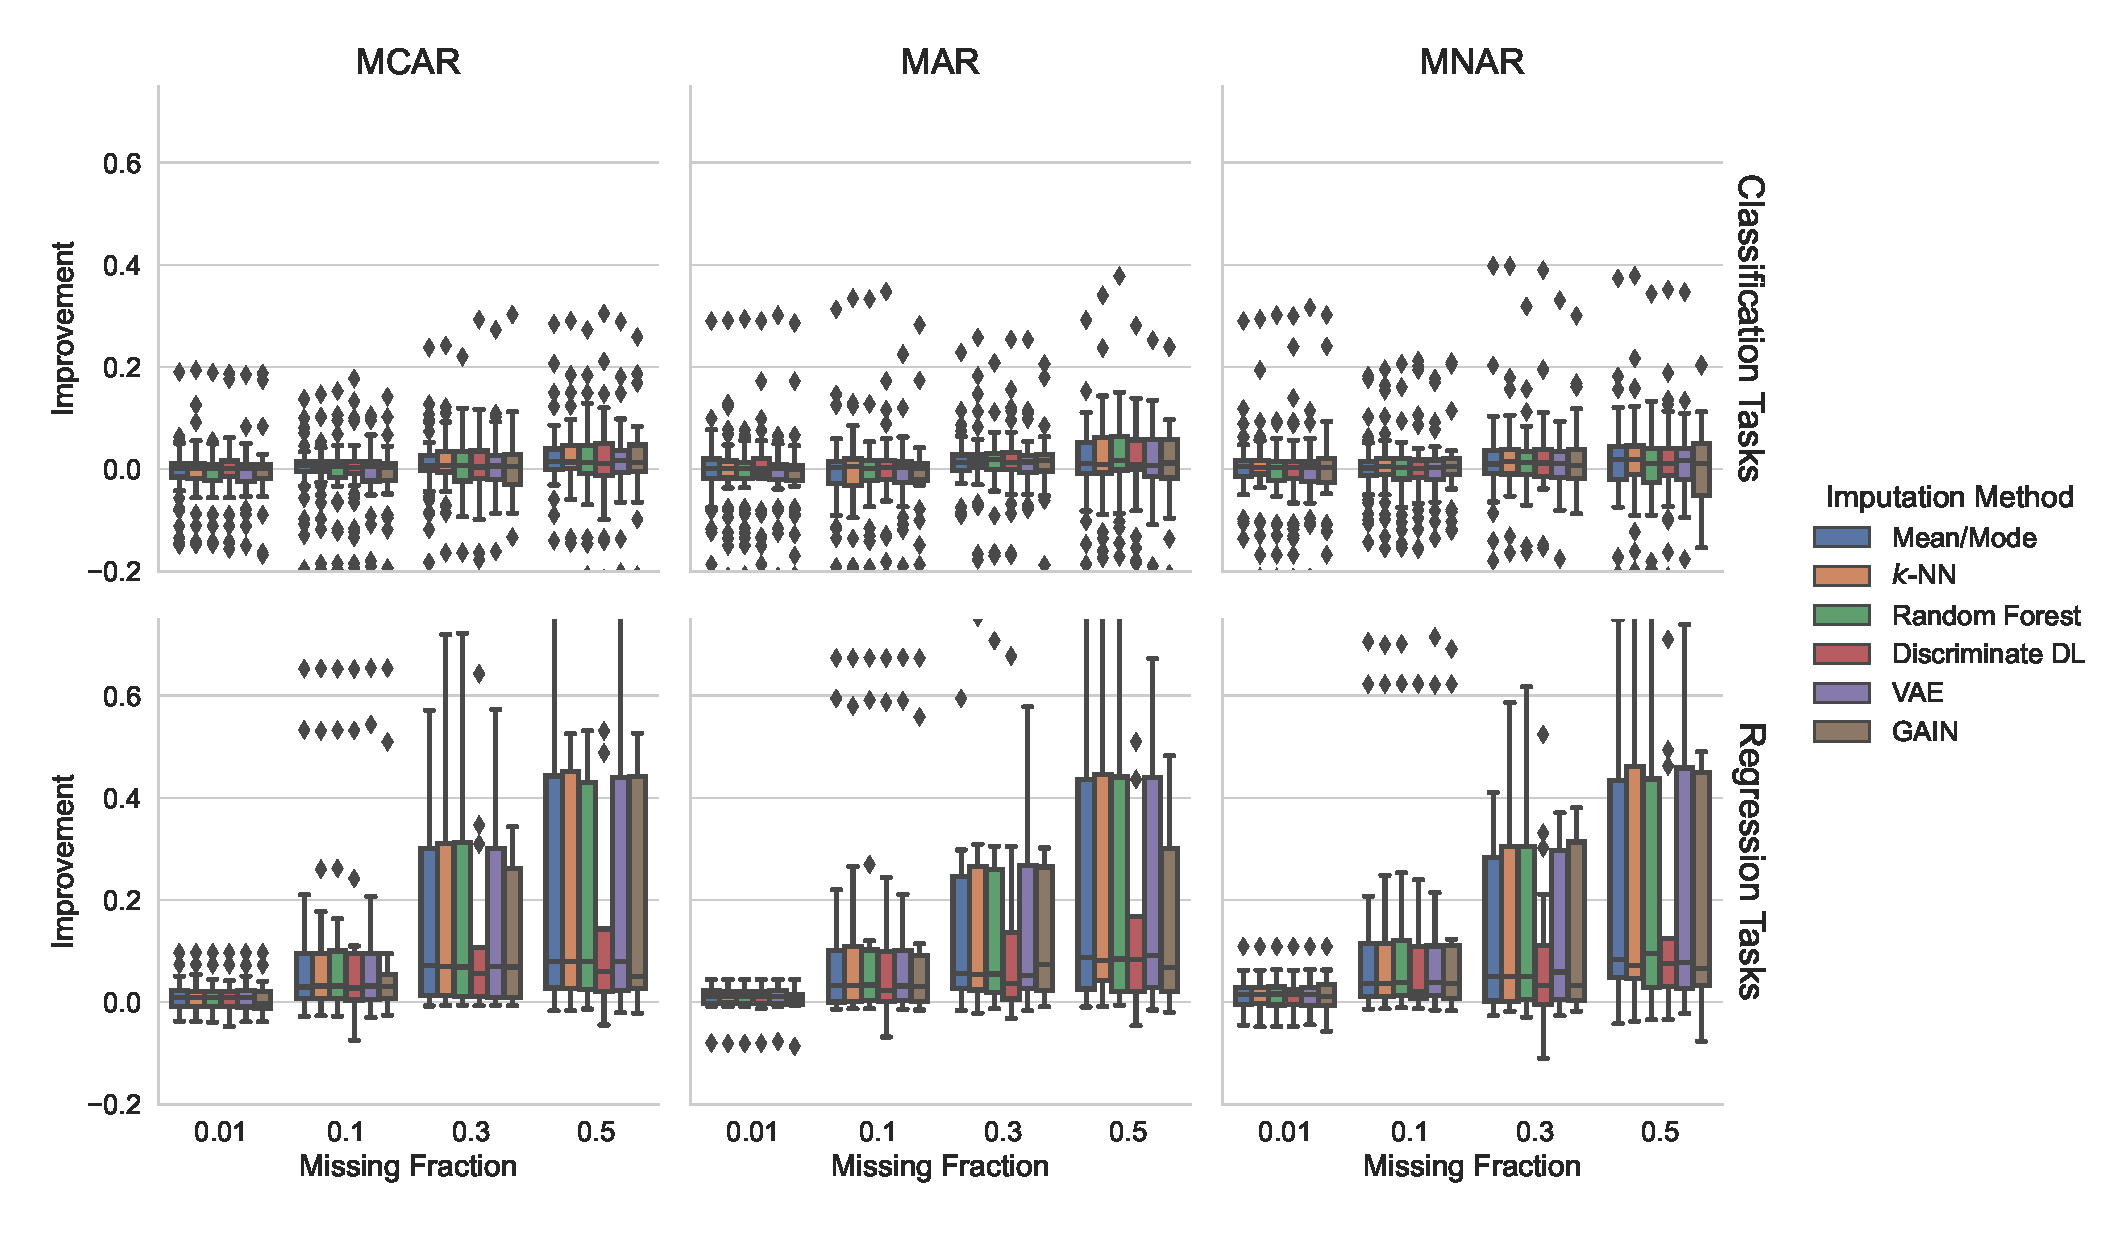
\includegraphics[width=1\columnwidth]{fully_observed_downstream_boxplot.eps}

	\caption[Downstream Ranks - Fully Observed]{In this figure, we visualize the results of \textit{Experiment 2} (impact on downstream task) in the \textit{Scenario 1} setting (training on complete data). The downstream improvement is plotted against the missingness fraction. The plot is divided into six sub-plots, with three columns determined by the missingness type, ordered by task difficulty from easiest to hardest (MCAR, MAR, MNAR). In the first row of sub-plots we depict results of classification tasks, whereas the second row contains regression results. Within a single sub-plot, each box represents the distribution of the \textit{impact on downstream task} metric (Equation \ref{eq:impact}) of a single imputer over all corresponding datasets/columns. Overall, the classical ML methods and discriminative DL perform best.
    }
	\label{fig:fully_observed_downstream_boxplot}
\end{figure}

Figure \ref{fig:fully_observed_downstream_boxplot} visualizes the \textit{impact on downstream task} metric (Equation \ref{eq:impact}) in \textit{Scenario 1}. \arndt{hier ggf. in einem Satz nochmal zusammenfassen, wie die Berechnung erfolgt (sinngemäß).}

The impact of imputation seems mostly negligible if the proportion of missing values is only 1\%. However, for numeric columns, there are some outliers in the 20\% to 40\% improvement range with the MCAR and MAR patterns at 1\% missing values. With an increasing proportion of missing values we observe increasing improvements in the downstream performance in all types of missingness patterns. However, there are also some cases where downstream performance is degraded by imputation, which is mainly the case for categorical columns.

For categorical columns, improvements are mostly in the 0\% to 5\% range, and in case of 50\% missing values the upper quartile reaches the 5\% to 10\% range. The whiskers even indicate performance increases which go significantly beyond. Measured by the median, as an overall aggregation, Random Forest yields the best results for categorical columns. GAIN performs often similarly well or even better but also has more negative fluctuations.

The situation is different for regression tasks. Here, GAIN clearly yields the least improvements downstream. Even the Mean imputation is oftentimes significantly more beneficial for the downstream tasks. The VAE results are approximately on par with Mean imputation. In contrast, the classical ML and the discriminative DL approaches do outperform the other methods in most settings. However, when the missing values are MNAR there is no clear advantage except that the discriminative DL is superior at 50\% missing values.

Overall, the classical ML methods and discriminative DL perform best. As the proportion of missing values increases, we observe increasing improvements in all types of missingness patterns, along with higher variance, in downstream performance. In contrast to classification tasks, there are hardly any negative effects in regression tasks.

\subsubsection{Scenario 2: Training on Incomplete/Imputed Data}


\begin{figure}\centering
	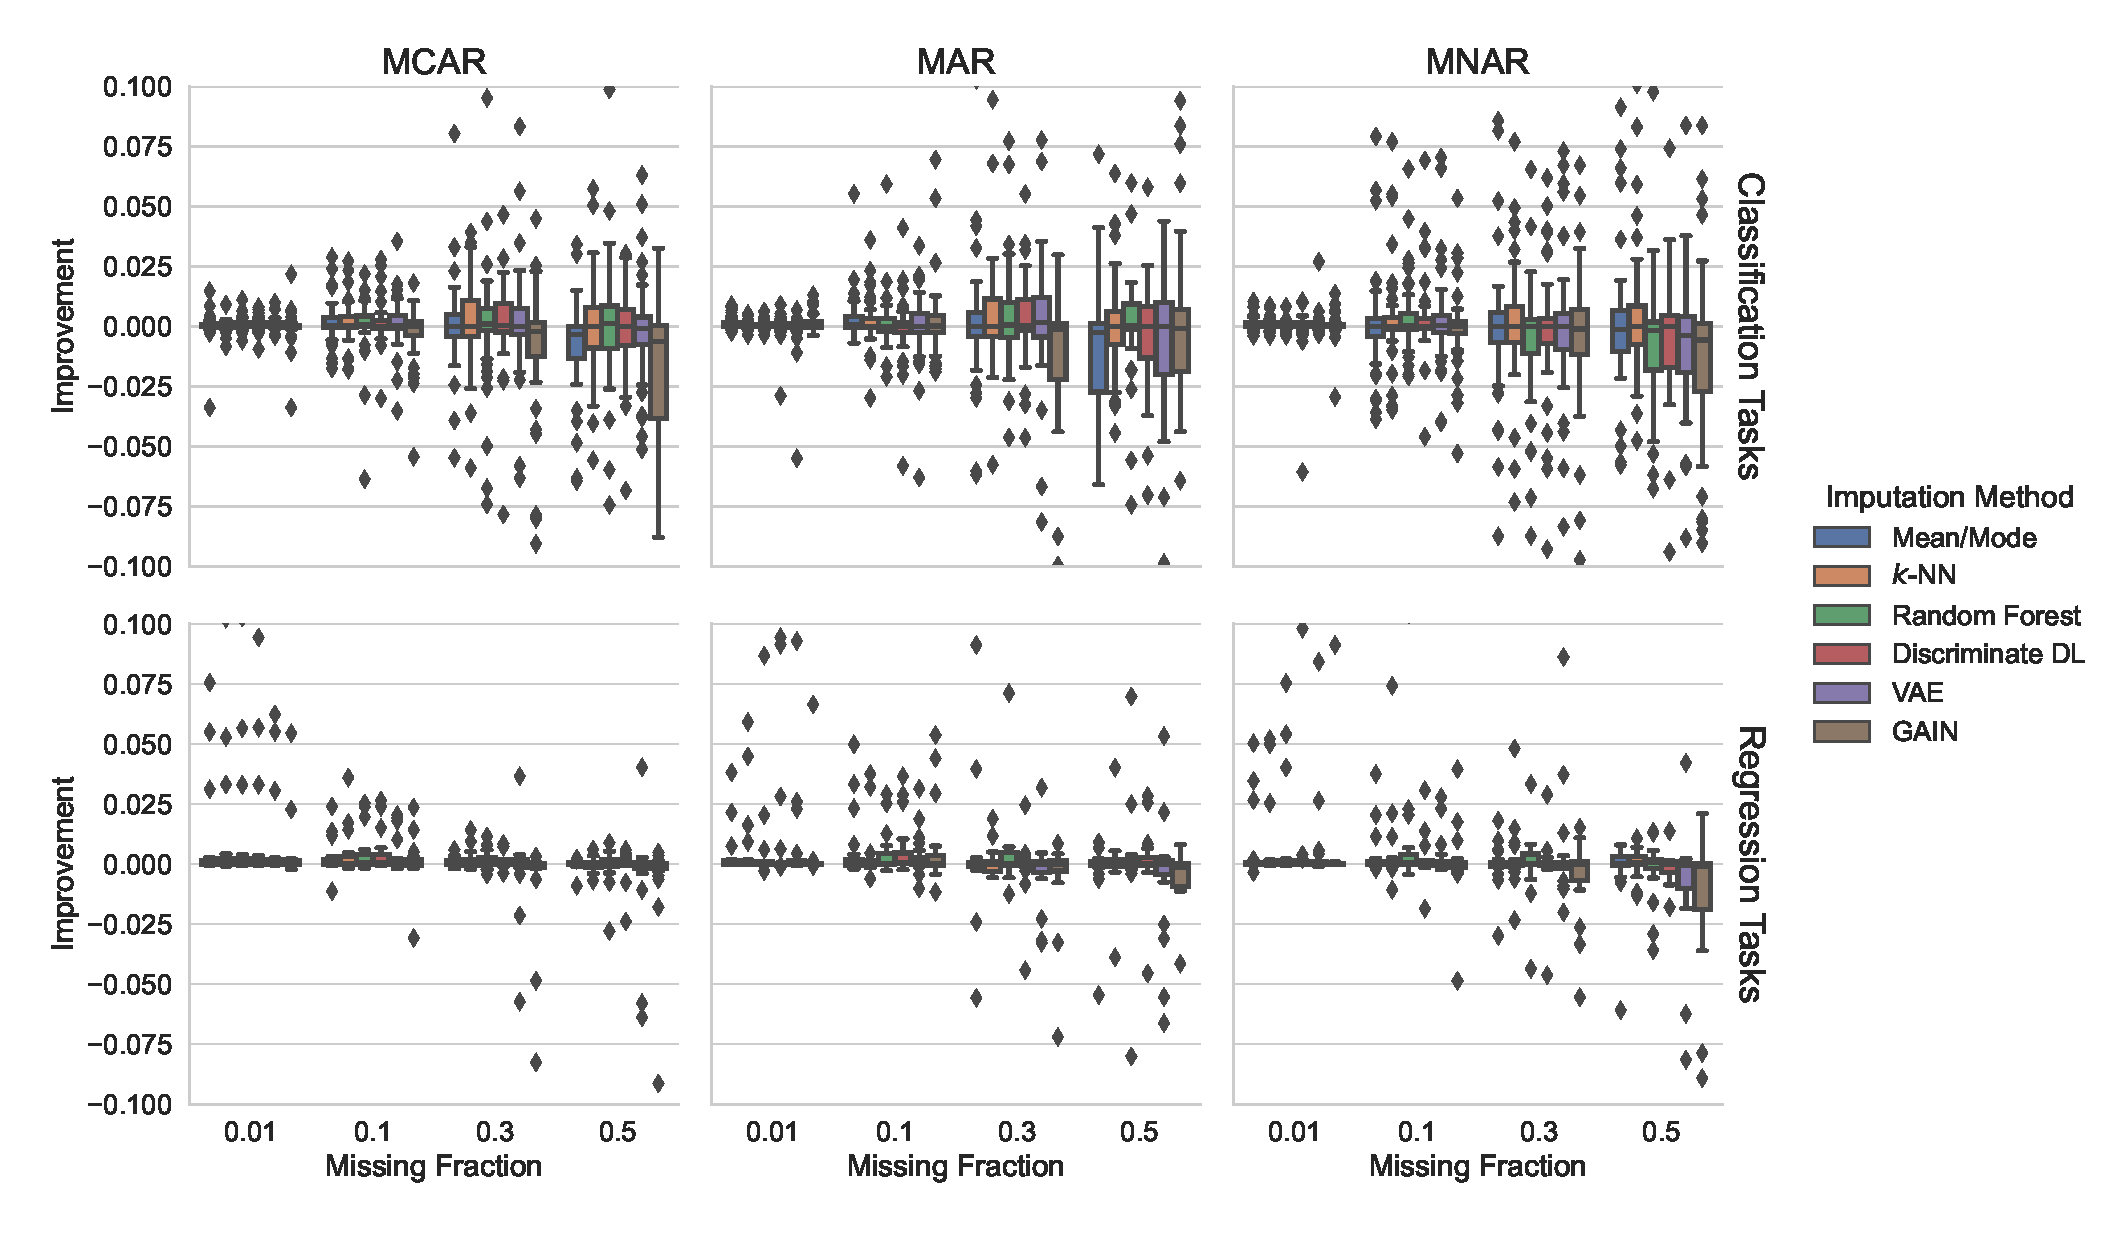
\includegraphics[width=1\columnwidth]{corrupted_downstream_boxplot.eps}

	\caption[Downstream Ranks - Corrupted]{In this figure, we visualize the results of \textit{Experiment 2} (impact on downstream task) in the \textit{Scenario 2} setting (training on incomplete/imputed data). The downstream improvement is plotted against the missingness fraction. The plot is divided into six sub-plots, with three columns determined by the missingness type, ordered by task difficulty from easiest to hardest (MCAR, MAR, MNAR). In the first row of sub-plots we depict results of classification tasks, whereas the second row contains regression results. Within a single sub-plot, each box represents the distribution of the \textit{impact on downstream task} metric (Equation \ref{eq:impact_scenario2}) of a single imputer over all corresponding datasets/columns. No considerable improvements were achieved in regression tasks. In classification tasks, there are slightly positive effects in some settings but negative effects predominate in the harder settings.
    }
	\label{fig:corrupted_downstream_boxplot}
\end{figure}

Figure \ref{fig:corrupted_downstream_boxplot} illustrates the \textit{impact on downstream task} (Equation \ref{eq:impact_scenario2}) in \textit{Scenario 2} (training on incomplete/imputed data). Here, the different scaling of the y-axis must be taken into account, i.e. the relative improvements are significantly smaller compared to the first scenario. One reason for this is the different basis for calculating the relative values (see sections \ref{sec:experiment_2} and \ref{sec:scenario_2}). \arndt{@Sebastian vllt. magsts du das noch mit einem weiteren Satz ausführen?!}

If weak positive effects seem to predominate in classification tasks at first, this tendency changes with increasing proportion of missing values (at 50\%) and increasing difficulty of the task (especially MNAR). The most negative results are produced by GAIN. However, the other methods also have major difficulties and often drift into negative ranges for the greater part as the tasks become more challenging.

In regression tasks, apart from a few outliers, there are no significant improvements. At the highest proportion of missing values (50\%) and greatest difficulty (MNAR), the results of the generative methods (VAE and GAIN) even turn predominantly negative.

In summary, no considerable improvements were achieved in regression tasks. In classification tasks, the picture is more mixed and the variance is higher. In some settings, there are slightly positive effects to note. In the difficult settings, however, the negative effects predominate.


\subsection{Training Time}

\begin{table}
	\centering
	\label{tab:time}
	\begin{tabular}{lrr}
		\toprule
		Imputation Method &  Training Time &  Relative Standard Deviation \\
		\midrule
		Mean/Mode &       0.005009 &                     0.656056 \\
		$k$-NN &      40.961577 &                     0.243020 \\
		Random Forest &     225.513999 &                     0.118707 \\
		Discriminative DL &    6285.017741 &                     0.424011 \\
		VAE &      71.685278 &                     0.107189 \\
		GAIN &     874.657293 &                     0.299608 \\
		\bottomrule
	\end{tabular}
	\caption{Training time for each imputation method in seconds. Training time is the mean overall experimental settings, experiments, and scenarios. The data set's size skews the standard deviation heavily, which is why we first compute the relative standard deviation for each imputation method on each data set separately and then average over the data sets.\felix{for knn the training time should be almost 0, right? maybe it would be good to have the inference/prediction times as well, if we have that? kNN should perform much worse here, and the winner should be RF, i'm assuming}}
\end{table}
